\documentclass[12pt,a4paper]{article}
\usepackage[utf8]{inputenc}
\usepackage[russian]{babel}
\usepackage{graphicx}
\usepackage{amsmath}
\usepackage[labelsep=period]{caption}
\textwidth=18cm
\oddsidemargin=-1.04cm
\headheight=0cm
\headsep=0cm
\topmargin=-1.04cm
\flushbottom
\setlength{\textheight}{50\baselineskip}
\setlength{\textheight}{\baselinestretch\textheight}
\addtolength{\textheight}{\topskip}


%\author{Капитонов А.А.,\\ассистент каф.~СУиИ \and Антонов Е.С.\\инженер каф.~СУиИ}
\title{Вопросы для защиты лабораторных работ по дисциплине <<Введение в специальность>>}
%\date{Санкт-Петербург\\осень--зима 2016 г.}
\date{}
\author{}
\begin{document}
\maketitle
\thispagestyle{empty}
\pagestyle{empty}

\subsection*{Лабораторная №1}
\begin{enumerate}
\item Назвать составные части двигателя постоянного тока. Указать, какие физические величины, описывающие состояние последнего, обозначены в работе как $J$, $\theta(t)$, $\omega(t)$, $\varepsilon(t)$, $M_\Sigma(t)$, $M_{el}(t)$ и $M_{oth}(t)$ и как они соотносятся друг с другом.
\item Для одной из функций, описывающих разгон ненагруженного двигателя постоянного тока ($\omega(t)$, $\theta(t)$ или $\varepsilon(t)$), написать ее аналитическое выражение, нарисовать график и отметить, как на внешнем виде последнего сказываются величины $\omega_{nls}$ и $T_m$. Конкретная функция, которая указанным образом должна быть описана студентом при защите, выбирается преподавателем.

Пример-пояснение:\\
При выборе преподавателем функции $\omega(t)$ студент в качестве ответа должен привести формулу (24) и график (со всеми подписями), представленный на рис.~2 методических указаний к работе.
\item Привести формулу для расчета величины $T_m$. Назвать входящие в нее величины.
\item Нарисовать схему моделирования процесса, описываемого заданным преподавателем дифференциальным уравнением.

Пример-пояснение:\\
При получении от преподавателя дифференциального уравнения
$$
y^{(3)} + a_1\dot{y} + a_2y = b
$$
студент должен изобразить схему моделирования, представленную на риc.~\ref{fig:modeling_scheme}.
\begin{figure}[h]
	\noindent\centering{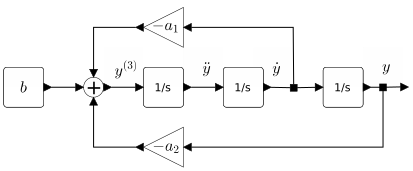
\includegraphics[scale=1.0]{modeling_scheme.pdf}}
	\caption{Требуемая схема моделирования.}
	\label{fig:modeling_scheme}
\end{figure}
\item Объяснить суть и цель аппроксимации экспериментальных данных некоторой функцией.
\end{enumerate}

\subsection*{Лабораторная №2}
\begin{enumerate}
\item Привести систему дифференциальных уравнений, описывающих работу двигателя постоянного тока. Пояснить все входящие в них физические величины и функции.\label{item:number_of_question_about_full_system}
\item Обозначить физический смысл конструктивных постоянных двигателя: рассказать между какими величинами, описывающими процесс работы двигателя постоянного тока, они устанавливают связь.
\item С~помощью системы уравнений из вопроса~\ref{item:number_of_question_about_full_system} нарисовать схему моделирования работы двигателя постоянного тока. Ответить на несколько дополнительных вопросов преподавателя, касающихся ее устройства.

Пример дополнительного вопроса:\\
Указать блок схемы, на выходе которого формируется значение силы тока, протекающего по обмоткам ротора двигателя.
\item Указать действия, применяемые для того, чтобы мотор NXT можно было рассматривать как обычный двигатель постоянного тока. 

Ключевые слова:\\
приведенный момент инерции, передаточное отношение редуктора.
\item Ответить на вопросы преподавателя, касающиеся работы с мультиметром в целом и измерению с его помощью силы тока и напряжения в частности.
\item Рассказать про метод наименьших квадратов в задаче аппроксимации экспериментальных данных некоторой функцией. Привести следующие из него формулы для расчета параметров $a$ и $b$ аппроксимирующих функций $y(x) = ax$ и $y(x) = ax + b$.
\end{enumerate}

\subsection*{Лабораторная №3}
\begin{enumerate}
\item Пояснить суть релейного регулятора, релейного регулятора с зоной нечувствительности и пропорционального регулятора. Для каждого из них привести описывающее его аналитическое выражения и изобразить график последнего.
\item Показать, как П-регулятор выглядит на используемой в работе схеме моделирования. Пояснить все формирующие его закон управления блоки.
\item Дать определения таким показателям качества систем управления, как перегулирование, время переходного процесса и ошибка управления. Найти численные значения для каждой из них, используя изображенный преподавателем график.
\item Рассказать, как в рассматриваемой в лабораторной задаче вышеуказанные показатели качества оказываются связанными со значением коэффициента П-регулятора. 
\end{enumerate}

\subsection*{Лабораторная №4}
\begin{enumerate}
\item Пояснить идею ПИД-регулятора. Указать, какие преимущества дают интегральная и дифференциальная составляющие.
\item Показать, как ПИД-регулятор выглядит на схеме моделирования. Пояснить все блоки, формирующие его закон управления.
\item Пояснить идею такого приема, как anti-windup. Рассказать, зачем он применяется.
\item Рассказать про методы численного:
\begin{itemize}
\item интегрирования:
а)~метод прямоугольников (правых, левых, средних);
б)~метод трапеций;
в)~метод парабол (метод Симпсона);
\item дифференцирования:
а)~метод односторонней (правой/левой) разности;
б)~метод двусторонней разности.
\end{itemize} 
\item Перечислить основные три типа приводов мобильных роботов. Указать преимущества, недостатки и возможности каждого из них.
\end{enumerate}

\subsection*{Лабораторная №5}
\begin{enumerate}
\item Решить заданное преподавателем линейное однородное или неоднородное дифференциальное уравнение с постоянными коэффициентами, прибегая при этом к решению его характеристического уравнения.

Примеры таких дифференциальных уравнений:
$$
2\ddot{y}-5\dot{y}+3y=5,\qquad\qquad \dddot y-3\ddot{y}+3\dot{y}-y=0\ldotp
$$
\item Для заданной преподавателем квадратной матрицы найти ее характеристический полином (многочлен).
\item Рассказать про модели объектов управления: про модель вход-выход (ВВ) и модель вход-состояние-выход (ВСВ).
\item Рассказать о матрице управляемости и ее роли в процессе разработки системы управления каким-либо объектом.
\item Пояснить идею П-регулятора состояния.
\item Привести формулу Аккермана. Указать, для чего она применяется.
\item Рассказать про алгоритм расчета коэффициентов П-регулятора состояния, который применялся в лабораторной работе.
\end{enumerate}

\subsection*{Общие замечания}
\begin{enumerate}
\item Необходимо знать единицы измерения каждой из физических величин, встречающихся в курсе. Их знание может быть проверено во время защиты любой из работ.
\end{enumerate}
\end{document}